\chapterimage{./Pictures/cover-writing}
\chapter{TP3: Configuration de serveur}
\textit{Le but de ce TP est d'utiliser le routeur afin de pouvoir configurer les machines s'y connectant automatiquement grâce au DHCP mais aussi de l'utiliser afin d'héberger des pages internet. Naturellement, ce TP suivant le TP2, la configuration est celle de celui-ci, et l'utilisation des scripts déterminés dans la fin de celui-ci ont permis la restauration rapide de l'architecture.}

\section{Mise en place d’un serveur DHCP}
\subsection{Comprendre le fonctionnement de DHCP}
Pour commencer, DHCP signifie Dynamic Host Configuration Protocol. Essentiellement, celui-ci permet à des machines se connectant au réseau où celui-ci est présent d'obtenir automatiquement une configuration valide pour un certain temps, et de récupérer les adresses des éventuels serveurs DNS ou de la passerelle par défaut.\\
Quant à son fonctionnement, celui-ci est simple, une machine nouvellement arrivé demande un "bail DHCP" en se signalant auprès de toutes les machines du réseau grâce à un message en diffusion. Le serveur écoutant le port approprié réagit alors en proposant une adresse IP via une offre DHCP au client (grâce à son adresse MAC), avec cette adresse est aussi précisé l'adresse IP du serveur et le masque de sous-réseau. Le client choisi une offre et répond positivement au serveur DHCP, celui-ci répond alors avec la durée du bail, ainsi que l'adresse IP effective que le client utilisera.

\subsection{Définition des paramètres du serveur DHCP}
Dans notre situation, la machine-routeur fera office de serveur DHCP, elle configurera la machine cliente normalement présente sur l'interface enp7s4. Il communiquera l'adresse IP que peut prendre prendre le client (les adresses utilisables se trouvant de 192.168.7.2 à 192.168.7.254), le masque de sous-réseau, ainsi que la passerelle par défaut (lui-même), l'adresse de diffusion (192.168.7.255).

\subsection{Mise en place duavec  serveur}
Afin d'installer le package concernant l'installation du serveur DHCP, on utilise la commande

\begin{minted}{bash}
apt install isc-dhcp-server
\end{minted}

On va aussi configurer les paramètres dans \textit{/etc/default/isc-dhcp-server}, en précisant l'interface utilisée dans la ligne:

\begin{minted}{bash}
INTERFACESv4="enp7s4"
\end{minted}

On configure ensuite le fichier \textit{/etc/dhcp/dhcpd.conf}, celui-ci est fourni

\inputminted[linenos]{bash}{../sources/TP3/server/dhcp/dhcpd.conf}

Afin de vérifier que tout fonctionne, on redémarre la machine cliente et on voit quelle configuration celle-ci prend. On voit que tout se passe correctement et qu'elle est configurée de façon adéquate.\\
Pour s'assurer qu'il s'agit bien du DHCP fonctionnant correctement, on utilise \textit{wireshark} pour surveiller les paquets échangés. Ce logiciel nous confirme qu'il y a bien eu échange de paquets DHCP. Voici les paquets identifiés:

\begin{figure}[H]
\centering
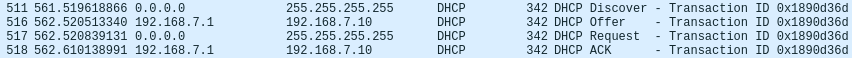
\includegraphics[width=400pt]{./TP3/Pictures/DHCP}
\caption{DHCP}
\label{DHCP}
\end{figure}

\section{Mise en place d’un serveur Web + SQL}
\subsection{Installation des packages}
Pour installer un serveur web apache, rien de plus simple, on commence par lancer la commande:
\begin{minted}{shell}
sudo apt install apache2 php mysql-server libapache2-mod-php php-mysql
\end{minted}
Il s'agit de tout les paquets nécessaires au bon fonctionnement du serveur, ainsi que l'utilisation d'une base de données et l'interaction Apache mySQL grâce au langage PHP.

\subsection{Mise en place du serveur Apache2}
Une fois le serveur Apache2 correctement installé, il nous faut maintenant le configurer. Dans notre cas, la configuration par défaut fonctionne très bien, on s'en contentera, tout en gardant à l'esprit les diverses nécessités de configuration pouvant survenir sur d'autres machines. Pour vérifier que tout marche, on se connecte simplement à l'adresse 127.0.0.1 sur un navigateur web. Une pageApache2 s'affiche, c'est que tout fonctionne.\\
Bien qu'il soit intéressant de pouvoir lire la page de configuration par défaut d'Apache2 dans un navigateur, il est plus pertinent d'y afficher un contenu choisi, en l'occurrence, une page HTML écrite par nos soins.Pour les besoin du TP, on utilisera simplement l'échantillon d'HTML fourni que l'on mettra dans \textit{/var/www/html/test.html}. Il suffit de se connecter à 127.0.0.1/test.html pour vérifier que cela a bien marché.

\begin{figure}[H]
\centering

\includegraphics[width=200pt]{./TP3/Pictures/index}
\caption{Index}
\label{Index}
\end{figure}

\subsection{Mise en place du serveur mySQL}
Nous avons déjàinstallé le paquet concernant mySQL dans la première partie. On utilise \textit{service mysql status} afin de savoir si celui-ci est en cours. Afin de pouvoir y accéder, on doit utiliser la commande \textit{mysql -u root}. Il peut arriver que l'installation n'est pas requise de mot de passe pour pouvoir accéder à l'utilisateur root de mySQL. Afin de régler ce problème, nous avons suivi cette procédure, trouvé grâce à l'aide de Google et de notre professeur de TP.

% Figure Debug mysql
\begin{figure}[H]
\centering
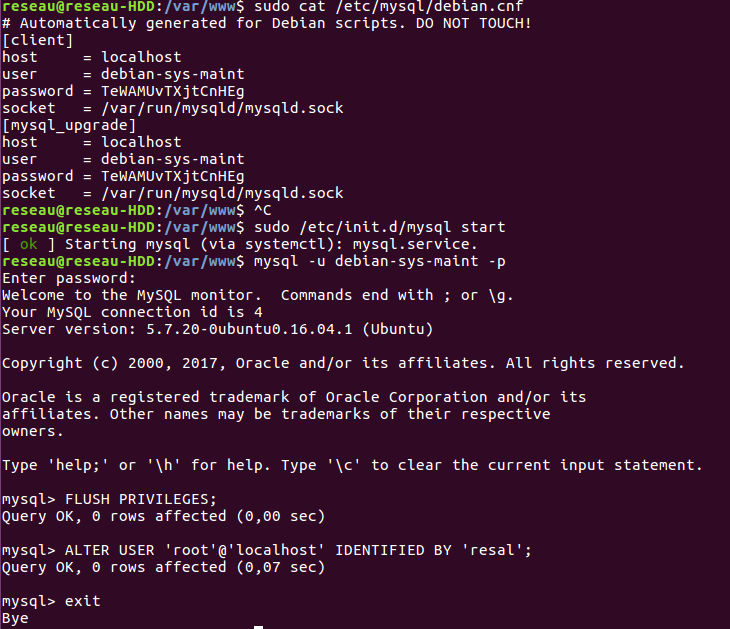
\includegraphics[width=400pt]{./TP3/Pictures/debug_mysql}
\caption{Debug mysql}
\label{Debug mysql}
\end{figure}

\subsection{Interaction mySQL et Apache}
Pour finir, nous installons \textit{phpMyAdmin} et \textit{WordPress} sur le serveur Apache. Afin d'automatiser ce processus, nous avons écrit un script permettant de réaliser les étapes nécessaires,

\inputminted[linenos]{bash}{../sources/TP3/server/LAMP/lamp.sh}

Ce script définit d'abord les emplacement des fichiers téléchargés et du répertoire où nous devons déployer les deux logiciels. Ensuite, il procè
de au télechargement des archives des logiciels, ainsi qu'à l'extraction de ceux-ci dans le répertoire /html/ d'apache.
